\documentclass[22pt]{article}
\title{\Huge {\vspace{-2cm}Solved zero energy model in topological superconductor}}
\author{\LARGE {Wei Cheng}}
\date{}
\usepackage{color}
\usepackage{verbatim}
\usepackage[UTF8]{ctex}%用于识别中文
\usepackage{underscore}%可以用来正确识别_
\usepackage{graphicx}%用于插入图片
\usepackage{color}
\usepackage{geometry}
\usepackage{braket}
\usepackage{listing}
\geometry{a4paper,scale=0.9}
\usepackage{hyperref}%用于插入链接
\hypersetup{
	colorlinks=true,
	linkcolor=blue,
	filecolor=magenta,      
	urlcolor=blue,
}%插入链接的性质
\usepackage{pythontex}
\usepackage{import}
\usepackage{xifthen}
\usepackage{pdfpages}
\usepackage{transparent}
\usepackage{framed}
\usepackage[dvipsnames,svgnames]{xcolor}
\usepackage[strict]{changepage}
\usepackage{xcolor}
\usepackage{soul}
\usepackage{abstract}
\usepackage{amsmath,amsthm,amssymb,amsfonts, fancyhdr, color, comment, graphicx, environ}
\renewcommand{\abstractname}{\LARGE Abstract}
\usepackage{titlesec}
\definecolor{mygreen}{rgb}{0.8,1,0.73}
\definecolor{linegreencolor}{rgb}{0,0.4,0}
\definecolor{myblue}{rgb}{0.22,0.73,0.91}


\titleformat*{\section}{\LARGE\bfseries}
\titleformat*{\subsection}{\LARGE\bfseries}
\titleformat*{\subsubsection}{\LARGE\bfseries}


\newenvironment{greenbox}{%
	\def\FrameCommand{%
		\hspace{1pt}%
		{\color{linegreencolor}\vrule width 2pt}%
		{\color{mygreen}\vrule width 4pt}%
		\colorbox{mygreen}%
	}%
	\MakeFramed{\advance\hsize-\width\FrameRestore}%
	\noindent\hspace{-4.55pt}% disable indenting first paragraph
	\begin{adjustwidth}{}{7pt}%
		\vspace{2pt}\vspace{2pt}%
	}
	{%
		\vspace{2pt}\end{adjustwidth}\endMakeFramed%
}
\newenvironment{bluebox}{%
	\def\FrameCommand{%
		\hspace{1pt}%
		{\color{myblue}\vrule width 2pt}%
		{\color{myblue}\vrule width 4pt}%
		\colorbox{myblue}%
	}%
	\MakeFramed{\advance\hsize-\width\FrameRestore}%
	\noindent\hspace{-4.55pt}% disable indenting first paragraph
	\begin{adjustwidth}{}{7pt}%
		\vspace{2pt}\vspace{2pt}%
	}
	{%
		\vspace{2pt}\end{adjustwidth}\endMakeFramed%
}


\newcommand{\incfig}[1]{%
	\def\svgwidth{\colum\left( nwidth}
	\import{./images/}{#1.pdf_tex}
}






\begin{document}
	\Large
	\maketitle
	\section*{The model}
	$H_{TI}(k)=M(k)\tau_3\sigma_0+A_1k_x\tau_2\sigma_1-A_1k_y\tau_2\sigma_2+A_1k_z\tau_2\sigma_3$,其中
	\par $M(k)=M_0+M_1(k_x^2+k_y^2)+M_2k_z^2$,其中$\tau$表示轨道,$\sigma$表示自旋。
	\begin{figure}[ht]
		\centering
		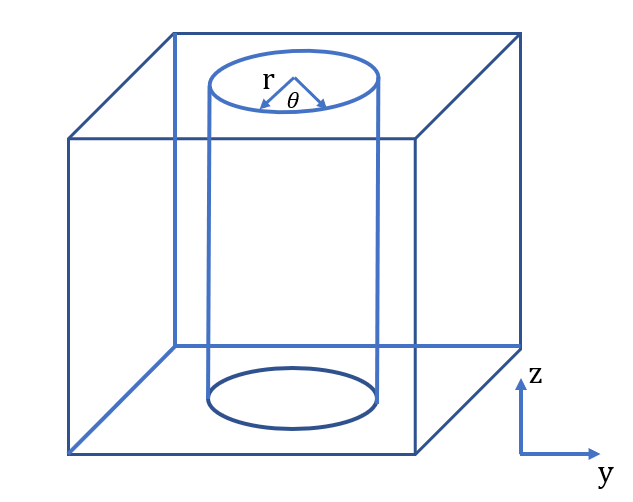
\includegraphics[scale=0.5]{Picture/1}
	\end{figure}
考虑在z方向加vortex,xy平面不在具有平移对称性,但z方向仍然有。其反带的点在$k_z=0或\pi$在此点处变成一个二维的哈密顿量。然后考虑随着化学势的变化其出现的一个拓扑相变,然后判断其其拓扑相变点位于$C_{2z}$的哪个本征值。推导的基本思路是将$BdG$哈密顿量投影到费米面附近的两条能带上,同时将角动量也投影过去。然后发现投影之后的角动量为整数,而且由于$k_y$系数的差异会相差1.而所要求解的哈密顿量通过一些变换可变为Jackiw-Rebbi model,由此便可以得到其零能束缚态的解所出现的位置。最终得到的结论是当$k_y$系数变号时,其相变位置的角动量会相差1.



	\begin{align}
		H_{TI}(k)=
		\begin{pmatrix}
			M(k) & && -iA_1k_{+}\\
			&M(k) &-iA_1k_{-} &\\
			&iA_1k_{+} &-M(k) &\\
			iA_1k_{-} & & &-M(k)
		\end{pmatrix}
	\end{align}
	易知$[\tau_3\sigma_3,H]=0$,故可在$\tau_3\sigma_3$的本征态中将其分块对角,可得
	\begin{align}
		U=
		\begin{pmatrix}
			1 &0&0&0\\
			0&0&1&0\\
			0&0&0&1\\
			0&1&0&0
		\end{pmatrix}
	\end{align}
	可得
	\begin{align}
		U^{\dagger}HU=
		\begin{pmatrix}
			M(k) & -iA_1k_{+} &&\\
			iA_1k_{-}&-M(k) &&\\
			&&M(k) &-iA_1k_{-}\\
			&&iA_1k_{+}&-M(k)
		\end{pmatrix}
	\end{align}
	分别求解每个对角块的情况
	\begin{align}
		\begin{pmatrix}
			M(k) &-iA_1k_{+}\\
			iA_1k_{-} &-M(k)
		\end{pmatrix}
		=M(k)\sigma_3+A_1k_x\sigma_2+A_1k_y\sigma_1
	\end{align}
	可知其两个本征值为$E_{\pm}(k)=\pm\sqrt{M(k)^2+A_1^2k_x^2+A_1^2k_y^2}$
	其两个本征值为
	\begin{align}
		\psi_{1+}=\frac{1}{\alpha_{+}(k)}
		\begin{pmatrix}
			E_{+}(k)+M(k)\\
			A_1k_y+iA_1k_x
		\end{pmatrix}
		\qquad
		\psi_{1-}=\frac{1}{\alpha_{-}(k)}
		\begin{pmatrix}
			E_{-}(k)+M(k)\\
			A_1k_y+iA_1k_x
		\end{pmatrix}
	\end{align}
	其中$\alpha_{\pm}(k)=\sqrt{(E_{\pm}+M(k))^2+A_1k_x^2+A_1k_y^2}$为归一化常数。
	
	\begin{align}
		\begin{pmatrix}
			M(k) &-iA_1k_{-}\\
			iA_1k_{+} &-M(k)
		\end{pmatrix}
		=M(k)\sigma_3+A_1k_x\sigma_2-A_1k_y\sigma_1
	\end{align}
	其两个本征值为$E_{\pm}=\pm\sqrt{M(k)^2+A_1^2k_x^2+A_1^2k_y^2}$,其两个本征态为
	\begin{align}
		\psi_{2+}=\frac{1}{\alpha_{+}(k)}
		\begin{pmatrix}
			E_{+}(k)+M(k)\\
			-A_1k_y+iA_1k_x
		\end{pmatrix}
		\qquad
		\psi_{2-}=\frac{1}{\alpha_{-}(k)}
		\begin{pmatrix}
			E_{-}(k)+M(k)\\
			-A_1k_y+iA_1k_x
		\end{pmatrix}
	\end{align}
	其中$\alpha_{\pm}(k)=\sqrt{(E_{\pm}+M(k))^2+A_1k_x^2+A_1k_y^2}$为归一化常数。
	将其写到极坐标系下可得
	\begin{align}
		\psi_{1+}=\frac{1}{\alpha_{+}(k)}
		\begin{pmatrix}
			\beta(k)\\
			iA_1ke^{-i\theta}\\
			0\\
			0
		\end{pmatrix}
		\qquad
		\psi_{2+}=
		\frac{1}{\alpha_{+}(k)}
		\begin{pmatrix}
			0\\
			0\\
			\beta(k)\\
			iA_1ke^{i\theta}
		\end{pmatrix}
	\end{align}
	将其变换到原来的基矢中,因为基矢做了一个$U$的变换,态矢量做了一个$U^{\dagger}$的变换,因此在态矢量前乘以一个$U$即可变回原来的态矢,可得
	\begin{align}
		\ket{\psi_{1+}}=\frac{1}{\alpha_{+}(\rho)}
		\begin{pmatrix}
			\beta(\rho)e^{(j+\frac{1}{2})\theta}\\
			0
			\\
		0\\
				iA_1\rho e^{(j-\frac{1}{2})\theta}
		\end{pmatrix}
		\ket{\psi_{2+}}=\frac{1}{\alpha_{+}(\rho)}
		\begin{pmatrix}
			0\\
			\beta(\rho)e^{(j-\frac{1}{2})\theta}\\
			iA_1\rho e^{(j+\frac{1}{2})\theta}
			\\
			0
		\end{pmatrix}
	\end{align}
	由于波函数可以有一个相位差,同时考虑到波函数的单值性,其两个本征态可写为
	\begin{align}
		\ket{\psi_{1+}}=\frac{1}{\alpha_{+}(k)}
		\begin{pmatrix}
			\beta(k)e^{in\theta}\\
			0
			\\
			0\\
			iA_1ke^{i(n-1)\theta}
		\end{pmatrix}
		\ket{\psi_{2+}}=\frac{1}{\alpha_{+}(k)}
		\begin{pmatrix}
			0\\
			\beta(k)e^{in\theta}\\
			iA_1ke^{i(n+1)\theta}
			\\
			0
		\end{pmatrix}
	\end{align}
其中n为整数。在此表象下,角动量$J_{ze}=-i\partial_{\theta}-\frac{1}{2}\sigma_3$,[这里$J_{ze}$下标表示电子部分沿着z方向的角动量,因为后面涉及到角动量比较多,这样写用于区分]写成矩阵形式为
\begin{align}
	J_{ze}=-i\partial_{\theta}-\frac{1}{2}
	\begin{pmatrix}
		1&&&\\
		&-1&&\\
		&&1&\\
		&&&-1
	\end{pmatrix}
\end{align}
可知
\begin{align}
	J_{ze}\ket{\psi_{1+}}=(n-\frac{1}{2})\ket{\psi_{1+}}  \qquad  J_{ze}\ket{\psi_{2+}}=(n+\frac{1}{2})\ket{\psi_{2+}}
\end{align}
由此可以看到$\ket{\psi_{1+}},\ket{\psi_{2+}}$均为$J_z$的本征态,为了方便,令$j=n-\frac{1}{2}$表示总角动量,易知其为半整数。现在再来考虑加上超导和vortex的情况。

	其空穴的哈密顿量为$-\sigma_2H_{-k}^{*}\sigma_2=-H(k)$
	由此电子部分和空穴部分为
	\begin{align}
		\nonumber
		\ket{\psi_1}_e=
		\begin{pmatrix}
			\ket{\psi_{1+}}\\
			0
		\end{pmatrix}
		\qquad
		\ket{\psi_2}_e=
		\begin{pmatrix}
			\ket{\psi_{2+}}
			\\
			0
		\end{pmatrix}
		\qquad
		\ket{\psi_1}_h=
		\begin{pmatrix}
			0\\
			\ket{\psi_{1+}}
		\end{pmatrix}
		\qquad
		\ket{\psi_2}_h=
		\begin{pmatrix}
			0\\
			\ket{\psi_{2+}}
		\end{pmatrix}
	\end{align}
现在将BdG哈密顿量投影到这四个基矢下,在基矢$(\Psi_k,\Psi_{-k}^{T}(i\sigma_2))$的BdG哈密顿量为
\begin{align}
	H_{BdG}=
	\begin{pmatrix}
		H_k-\mu &  H_{\Delta}  \\
		H_{\Delta}^{\dagger} & \mu-H_k
	\end{pmatrix}
\end{align}
其中
\begin{align}
	H_{\Delta}=
	\begin{pmatrix}
		\Delta(r) & & &\\
		&\Delta(r) & &\\
		&& \Delta(r) &\\
		&&&\Delta(r)
	\end{pmatrix}
\end{align}
考虑沿着z轴的vortex时,$\Delta_0\tanh(\frac{r}{\xi})e^{-i\theta}$表示,其中$\xi$表示超导的相干长度,$\theta$表示超导相位,当靠近vortex中心的时候,可以做一个小量展开,即$\tanh(\frac{r}{\xi})=\frac{r}{\xi}$,由此可以得到$\Delta(r)=\frac{\Delta_0}{\xi}re^{-i\theta}=\Delta_e(x-iy)$
\\
然后将其写到希尔伯特空间$\{\ket{\psi_1}_e,\ket{\psi_2}_e,\ket{\psi_1}_h,\ket{\psi_2}_h\}$,即计算矩阵元
\begin{align}
	e\bra{\psi_1}H_{BdG}\ket{\psi_1}_e=
	\begin{pmatrix}
		\bra{\psi_{1+}}&0
	\end{pmatrix}
	\begin{pmatrix}
	H_k-\mu &  H_{\Delta}  \\
	H_{\Delta}^{\dagger} & \mu-H_k
\end{pmatrix}
\begin{pmatrix}
	   \ket{\psi_{1+}}\\
	   0
\end{pmatrix}
=E_k-\mu
\end{align}
\begin{align}
	e\bra{\psi_1}H_{BdG}\ket{\psi_1}_h=\bra{\psi_{1+}}\Delta_e(x-iy)\ket{\psi_{1+}}=i\Delta_e(\partial_{k_x}-i\partial_{k_y}+A_{kx}^{11}-iA_{ky}^{11})
\end{align}
其中$A_x^{11}=i\bra{\psi_{1+}}\partial_{k_x}\ket{\psi_{1+}}$,继续计算其他矩阵元,最后可以得到
\begin{align}
	\nonumber
	\mathcal{H}_k^{BdG}=
	\begin{pmatrix}
		E(k)-\mu & \Delta_e[i\partial_{k_x}+\partial_{k_y}+A_{kx}^{\mu\nu}-iA_{ky}^{\mu\nu}]\\
		\Delta_e[i\partial_{k_x}-\partial_{k_y}+A_{kx}^{^{\mu\nu}}+iA_{ky}^{\mu\nu}] &\mu-E(k)
	\end{pmatrix}
\end{align}
其中$A_{kx}^{\mu\nu}=i\bra{\psi_{\mu+}}\partial_{kx}\ket{\psi_{\nu+}}$,同时可以考虑$J_{zv}$[这里下角标zv表示加上了vortex之后沿z方向的角动量]project到这个空间的形式$J_{z}=-i\partial_{\theta}+\frac{1}{2}\sigma_3+\frac{1}{2}s_3$[其中$\sigma$表示自旋,s表示particle-hole],写成矩阵形式就是
\begin{align}
	J_{zv}=J_{ze}+\frac{1}{2}s_3=
	\begin{pmatrix}
		J_{ze}+\frac{1}{2} &\\
		& J_{ze}-\frac{1}{2}
	\end{pmatrix}
\end{align}
然后将其投影到$\{\ket{\psi_1}_e,\ket{\psi_2}_e,\ket{\psi_1}_h,\ket{\psi_2}_h\}$空间,即分别计算其矩阵元可以得到$J_{zv}$的形式为
\begin{align}
	J_{zv}=
	\begin{pmatrix}
		n&&&\\
		&n+1&&\\
		&&n-1&\\
		&&&n
	\end{pmatrix}
	=n-\frac{1}{2}\sigma_3+\frac{1}{2}s_3
\end{align}


当这两条band可以用自旋加以区分时,$A_{kx}^{\mu\nu}$一定是一个对角的[严格的证明目前还无法给出],其形式为
\begin{align}
	H_{BdG}=
	\begin{pmatrix}
		E_k-\mu & &\Delta  &\\
		& E_k-\mu& & \Delta &\\
		\Delta^{\dagger} &    & \mu-E_k &\\
		& \Delta^{\dagger} && \mu-E_k
	\end{pmatrix}
\end{align}
可以做一个Unitary的变换,将其分块对角
\begin{align}
	U=
	\begin{pmatrix}
		1&0&0&0\\
		0&0&1&0\\
		0&1&0&0\\
		0&0&0&1
	\end{pmatrix}
\end{align}
\begin{align}
	U^{\dagger}H_{BdG}U=
	\begin{pmatrix}
		E_k-\mu &\Delta &&\\
		\Delta^{\dagger} &\mu-E_k &&\\
		&& E_k-\mu &\Delta \\
		&&\Delta^{\dagger}& \mu-E_k
	\end{pmatrix}
\end{align}
这个变换的实质是因为$\{\ket{\psi_1}_e,\ket{
\psi_1}_h\}$与$\{\ket{\psi_2}_e,\ket{
\psi_2}_h\}$之间没有耦合,因此可以project到这两个子空间进行求解,对于角动量而言有
\begin{align}
	U^{\dagger}J_{zv}U=n+
	\begin{pmatrix}
		0&&&\\
		&-1&&\\
		&&1&\\
		&&&0
	\end{pmatrix}
\end{align}
由此可知在$\{\ket{\psi_1}_e,\ket{\psi_1}_h\}$中$J_{z1-}=n-\frac{1}{2}+\frac{1}{2}\Pi_3$,在$\{\ket{\psi_2}_e,\ket{\psi_2}_h\}$中$J_{z2-}=n+\frac{1}{2}+\frac{1}{2}\Pi_3$
\\
当$k_y$前面的系数为正的时候,$J_z=-i\partial_{\theta}+\frac{1}{2}\sigma_3+\frac{1}{2}s_3$,用同样的方法project之后可以得到
\begin{align}
	U^{\dagger}J_{zv}U=n
	+
	\begin{pmatrix}
		1&&&\\
		&0&&\\
		&&0&\\
		&&&-1
	\end{pmatrix}
\end{align}
由此可以得到$J_{z1+}=n+\frac{1}{2}+\frac{1}{2}\Pi_3$\qquad$J_{z2+}=n-\frac{1}{2}+\frac{1}{2}\Pi_3$从这里便可以看出他们相对应的角动量差值为1.
现在来求解$BdG$哈密顿量
\begin{align}
	\nonumber
	\tilde{\mathcal{H}}_k^{BdG}=
	\begin{pmatrix}
		E(k)-\mu  & 
		\Delta_e[i\partial_{k_x}+\partial_{k_y}+A_{k_x}-iA_{k_y}]\\
		\Delta_e[i\partial_{k_x}-\partial_{k_y}+A_{k_x}+iA_{k_y}] & \mu-E(k)
	\end{pmatrix}
\end{align}
将其写到极坐标系下可得
\begin{align}
	\nonumber
	\tilde{\mathcal{H}}_k^{BdG}=
	\begin{pmatrix}
		E(k)-\mu  & \Delta_ee^{-i\theta}[i(\partial_k-i\frac{\partial_{\theta}}{k})+A_k-i\frac{A_{\theta}}{k}]\\
		\Delta_ee^{i\theta}[i(\partial_k+i\frac{\partial_{\theta}}{k})+A_k+i\frac{A_{\theta}}{k}] & \mu-E(k)
	\end{pmatrix}
\end{align}
其中$A_k,A_{\theta}$的大小是依赖于规范选择的,因此可以通过选择规范使其中一项为0,因为系统具有连续旋转对称性,对于同一个k,不同角度的$A_{\theta}$是相同的[选取$A_k=0$这个规范的理由还不够充分,还需进一步思考]。由$A_k=i\bra{\varphi_k}\partial_k\ket{\varphi_k}$,可知做一个规范变换$U=e^{i\int_0^{k}A_{k^{'}}dk^{'}}$,将其带入即会变成0.
由此可以得到此时的BdG哈密顿量变为
\begin{align}
	\tilde{\mathcal{H}}_k^{BdG}=
	\begin{pmatrix}
		E(k)-\mu  & i\Delta_ee^{-i\theta}(\partial_k-\frac{i\partial_{\theta}+A_{\theta}}{k})\\
		i\Delta_ee^{i\theta}(\partial_k+\frac{i\partial_{\theta}+A_{\theta}}{k})
		&  \mu-E(k)
	\end{pmatrix}
\end{align}
然后通过寻找一些对称性,分块对角这个哈密顿量。因为体系具有连续旋转对称性,因此可以定义一个effective的角动量$J_{zeff}$来进行求解,为了计算方便,将$\tilde{\mathcal{H}_k^{BdG}}$写成泡利矩阵的形式
\begin{align}
	\tilde{\mathcal{H}}_k^{BdG}&=(E(k)-\mu)\sigma_z+i\Delta_ee^{-i\theta}(\partial_k-\frac{i\partial_{\theta}+A_{\theta}}{k})\frac{1}{2}(\sigma_x+i\sigma_y)\\
	&+i\Delta_ee^{i\theta}(\partial_k+\frac{i\partial_{\theta}+A_{\theta}}{k})\frac{1}{2}(\sigma_x-i\sigma_y)\\
	&=(E(k)-\mu)\sigma_z+i\Delta_e(cos\theta\partial_k+isin\theta\frac{i\partial_{\theta}+A_{\theta}}{k})\sigma_x\\
	&+\Delta_e(isin\theta\partial_k+cos\theta\frac{i\partial_{\theta}+A_{\theta}}{k})\sigma_y
\end{align}
由此可以计算轨道角动量和H的对易子$[-i\partial_{\theta},\tilde{\mathcal{H}}_k^{BdG}]$
\begin{align}
	[-i\partial_{\theta},\tilde{\mathcal{H}}_k^{BdG}]&=[-i\partial_{\theta},i\Delta_e(cos\theta\partial_k+isin\theta\frac{i\partial_{\theta}+A_{\theta}}{k})\sigma_x]\\
	&+[-i\partial_{\theta},\Delta_e(isin\theta\partial_k+cos\theta\frac{i\partial_{\theta}+A_{\theta}}{k})\sigma_y]
\end{align}
\begin{align}
	&[-i\partial_{\theta},i\Delta_e(cos\theta\partial_k+isin\theta\frac{i\partial_{\theta}+A_{\theta}}{k})\sigma_x]
	\\&=[-i\partial_{\theta},i\Delta_ecos\theta\partial_k]\sigma_x+[-i\partial_{\theta},-\Delta_esin\theta\frac{i\partial_{\theta}+A_{\theta}}{k}]\sigma_x\\
	&=\Delta_e[\partial_{\theta},cos\theta\partial_k]\sigma_x+i\Delta_e[\partial_{\theta},sin\theta\frac{i\partial_{\theta}+A_{\theta}}{k}]\sigma_x\\ \nonumber
	&=\Delta_e(\partial_{\theta}(cos\theta\partial_k)-cos\theta\partial_k\partial_{\theta})\sigma_x+i\Delta_e(\partial_{\theta}(sin\theta\frac{i\partial_{\theta}+A_{\theta}}{k})-sin\theta\frac{i\partial_{\theta}+A_{\theta}}{k}\partial_{\theta})\sigma_x\\
	&=\Delta_e(-sin\theta\partial_k)\sigma_x+i\Delta_e(cos\theta\frac{i\partial_{\theta}+A_{\theta}}{k})\sigma_x \\
	&=i\Delta_e(isin\theta\partial_k+cos\theta\frac{i\partial_{\theta}+A_{\theta}}{k})\sigma_x
\end{align}
\begin{align}
	&[-i\partial_{\theta},\Delta_e(isin\theta\partial_k+cos\theta\frac{i\partial_{\theta}+A_{\theta}}{k})\sigma_y]\\
	&=\Delta_e[\partial_{\theta},sin\theta\partial_k]\sigma_y-i\Delta_e[\partial_{\theta},cos\theta\frac{i\partial_{\theta}+A_{\theta}}{k}]\sigma_y\\ \nonumber
	&=\Delta_e(\partial_{\theta}(sin\theta\partial_k)-sin\theta\partial_k\partial_{\theta})\sigma_y-i\Delta_e(\partial_{\theta}(cos\theta\frac{i\partial_{\theta}+A_{\theta}}{k})-cos\theta\frac{i\partial_{\theta}+A_{\theta}}{k}\partial_{\theta})\sigma_y\\
	&=\Delta_e(cos\theta\partial_k)\sigma_y-i\Delta_e(-sin\theta\frac{i\partial_{\theta}+A_{\theta}}{k})\sigma_y\\
	&=\Delta_e(cos\theta\partial_k+isin\theta\frac{i\partial_{\theta}+A_{\theta}}{k})\sigma_y
\end{align}
由此即可得到
\begin{align}
	\nonumber
	[-i\partial_{\theta},\tilde{\mathcal{H}}_k^{BdG}]=i\Delta_e(isin\theta\partial_k+cos\theta\frac{i\partial_{\theta}+A_{\theta}}{k})\sigma_x+\Delta_e(cos\theta\partial_k+isin\theta\frac{i\partial_{\theta}+A_{\theta}}{k})\sigma_y
\end{align}
\begin{align}
	\nonumber
	\tilde{\mathcal{H}}_k^{BdG}&=i\Delta_e(cos\theta\partial_k+isin\theta\frac{i\partial_{\theta}+A_{\theta}}{k})\sigma_x+\Delta_e(isin\theta\partial_k+cos\theta\frac{i\partial_{\theta}+A_{\theta}}{k})\sigma_y 
	\\&+(E(k)-\mu)\sigma_z
\end{align}
可以观察到$[-i\partial_{\theta},\tilde{\mathcal{H}}_k^{BdG}]$中$\sigma_x,\sigma_y$前面的系数与$\tilde{\mathcal{H}}_k^{BdG}$中$\sigma_y,\sigma_x$的系数差一个i,由泡利矩阵的对易关系$[\sigma_z,\sigma_x]=2i\sigma_y,[\sigma_z,\sigma_y]=-2i\sigma_x$,由此可以得到
\begin{align}
	\nonumber
	[\frac{1}{2}\sigma_z,\tilde{\mathcal{H}}_k^{BdG}]=-\Delta_e(cos\theta\partial_k+isin\theta\frac{i\partial_{\theta}+A_{\theta}}{k})\sigma_y-i\Delta_e(isin\theta\partial_k+cos\theta\frac{i\partial_{\theta}+A_{\theta}}{k})\sigma_x
\end{align}
由此可以定义一个effective的总角动量$J_{zeff}=l_z+\frac{1}{2}\Pi_z,[J_{zeff},\tilde{\mathcal{H}}_k^{BdG}]=0$,然后再来求解$J_{eff}$的本征函数,设$J_{zeff}\ket{\psi}=m\ket{\psi}$,即
\begin{align}
	\begin{pmatrix}
		-i\partial_{\theta}+\frac{1}{2} & \\
		& -i\partial_{\theta}-\frac{1}{2}
	\end{pmatrix}
	\begin{pmatrix}
		\psi_1\\
		\psi_2
	\end{pmatrix}
	=m
	\begin{pmatrix}
		\psi_1\\
		\psi_2
	\end{pmatrix}
\end{align}
\begin{align}
	(-i\partial_{\theta}+\frac{1}{2})\psi_1=m\psi_1 \\
	(-i\partial_{\theta}-\frac{1}{2})\psi_2=m\psi_2
\end{align}
可以得到
\begin{align}
	\psi_1=f_1(k)e^{i(m-\frac{1}{2})\theta} \\
	\psi_2=f_2(k)e^{i(m+\frac{1}{2})\theta}
\end{align}
设$l_z$的本征值为n,则可得$m=n\pm\frac{1}{2}$,考虑$m=n-\frac{1}{2}$,同时为了保证其厄米性,需要加入一个$\frac{1}{\sqrt{k}}$
\begin{align}
	\psi(k,\theta)=
	\frac{1}{\sqrt{k}}
	\begin{pmatrix}
		f_1(k)e^{i(n-1)\theta}\\
		-if_2(k)e^{in\theta}
	\end{pmatrix}
\end{align}
由此可以得到
\begin{align}
	\tilde{\mathcal{H}}_k^{BdG}\psi(k,\theta)=\varepsilon(k)\psi(k,\theta)
\end{align}
\begin{align}
	\nonumber
	\tilde{\mathcal{H}}_k^{BdG}
	\frac{1}{\sqrt{k}}
	\begin{pmatrix}
		e^{i(n-1)\theta} & \\
		&-ie^{in\theta}
	\end{pmatrix}
	\begin{pmatrix}
		f_1(k)\\
		f_2(k)
	\end{pmatrix}
	=\varepsilon(k)
	\frac{1}{\sqrt{k}}
	\begin{pmatrix}
		e^{i(n-1)\theta} & \\
		&-ie^{in\theta}
	\end{pmatrix}
	\begin{pmatrix}
		f_1(k)\\
		f_2(k)
	\end{pmatrix}
\end{align}
由此可以得到$\begin{pmatrix}
	f_1(k)\\
	f_2(k)
\end{pmatrix}$满足
\begin{align}
	\nonumber
	\sqrt{k}
	\begin{pmatrix}
		e^{-i(n-1)\theta} &\\
		&ie^{-in\theta}
	\end{pmatrix}
	\tilde{\mathcal{H}}_k^{BdG}
	\frac{1}{\sqrt{k}}
	\begin{pmatrix}
		e^{i(n-1)\theta} & \\
		&-ie^{in\theta}
	\end{pmatrix}
	\begin{pmatrix}
		f_1(k) \\
		f_2(k)
	\end{pmatrix}
	=\varepsilon(k)
	\begin{pmatrix}
		f_1(k) \\
		f_2(k)
	\end{pmatrix}
\end{align}
即$\begin{pmatrix}
	f_1(k)\\
	f_2(k)
\end{pmatrix}$的有效哈密顿量为
\begin{align}
	&
	\sqrt{k}
	\begin{pmatrix}
		e^{-i(n-1)\theta} &\\
		&ie^{-in\theta}
	\end{pmatrix}
	\tilde{\mathcal{H}}_k^{BdG}
	\frac{1}{\sqrt{k}}
	\begin{pmatrix}
		e^{i(n-1)\theta} & \\
		&-ie^{in\theta}
	\end{pmatrix}
	\\ \nonumber	
	&=	\sqrt{k}\begin{pmatrix}
		e^{-i(n-1)\theta} &\\
		&ie^{-in\theta}
	\end{pmatrix}
	\begin{pmatrix}
		E(k)-\mu  & i\Delta_ee^{-i\theta}(\partial_k-\frac{i\partial_{\theta}+A_{\theta}}{k})\\
		i\Delta_ee^{i\theta}(\partial_k+\frac{i\partial_{\theta}+A_{\theta}}{k})
		&  \mu-E(k)
	\end{pmatrix}
\\ \nonumber
& \qquad\qquad \qquad \qquad \qquad \qquad \qquad \qquad \qquad\qquad\qquad\qquad
\frac{1}{\sqrt{k}}
	\begin{pmatrix}
		e^{i(n-1)\theta} & \\
		&-ie^{in\theta}
	\end{pmatrix}\\  \nonumber
	\\ \nonumber
	&=\begin{pmatrix}
		E(k)-\mu &   \Delta_e[\partial_k+\frac{n-\frac{1}{2}-A_{\theta}}{k}] \\
		\Delta_e[\frac{n-\frac{1}{2}-A_{\theta}}{k}-\partial_k] & \mu-E(k)
	\end{pmatrix}
	\\ 
	&=[E(k)-\mu]\sigma_z+i\Delta_e\partial_k\sigma_y+\frac{\Delta_e}{k}(n-A_{\theta}-\frac{1}{2})\sigma_x
\end{align}

由此便可以得到$\begin{pmatrix}
	f_1(k) \\
	f_2(k)
\end{pmatrix}$的有效哈密顿量为
\begin{align}
	\tilde{\mathcal{H}}_j=[E(k)-\mu]\sigma_z+i\Delta_e\partial_k\sigma_y+\frac{\Delta_e}{k}(j-\frac{\phi_F}{2\pi})\sigma_x
\end{align}
在费米面附近可以得到
\begin{align}
	\varepsilon_n=\frac{\Delta_e}{k_{F}}(n-A_{\theta}^{k_{F}}-\frac{1}{2})
\end{align}
由于其具有连续旋转对称性,可以得到$A_{\theta}^{k_F}=\frac{\phi_F}{2\pi}$,即
\begin{align}
	\varepsilon_n=\frac{\Delta_e}{k_F}(j-\frac{\phi_F}{2\pi})
\end{align}
可知其中一个零能解出现在$\phi_F=\pi,n=1$处,$n$是$l_z$的本征值,即出现在$l_z=1$处,$m=\frac{1}{2}$,上面考虑的是$m=n-\frac{1}{2}$的情况,容易推得在$m=n+\frac{1}{2}$时,零能解出现在$n=0$,$m=\frac{1}{2}$处。即零能解出现在effective角动量为$\frac{1}{2}$的地方。对比effective角动量和投影之后的角动量的形式,可以得到$J_{z-}=J_{zeff}-\frac{1}{2}$,$J_{z+}=J_{zeff}+\frac{1}{2}$,[其中$\pm$表示$k_y$前面系数的正负。]即当$k_y$前面系数为负的时候$J_{z-}=m-\frac{1}{2}$由此其相变点会出现在$J_{z-}=0$处,当$k_y$前面系数为正的时候,$J_{z+}=m+\frac{1}{2}$,由此其相变点会出现在$J_{z+}=1$处。
\section*{Conclusion}
通过求解电子部分哈密顿量的本征态,得到了轨道角动量在$k_y$前面系数变号时会相差1这样一个结论。证明过程中还有一些不严格的点需要进一步思考,在确定effective角动量和总角动量之间的关系时,目前我想到的原因是其角动量的形式应该是一样的,因为他们投影的过程是完全一样的,但感觉不是很具体,后面需要从更具体的运算得到其相等关系。从目前的推导过程似乎分不出其相变点由于系数的正负的变化一个出现在角动量为奇数的部分,另一个出现在角动量为偶数的部分,似乎感觉只能确定其相变点是在$J_z$相差为1的不同本征值的地方。所以先尝试用Vishwanath后面讨论没有旋转对称性的方法试一试,后续再进行整理。
\end{document}